\documentclass[../memoire.tex]{subfiles}
\begin{document}

\chapter{Technical comparative analysis} \label{ch_snd}

\section{Architectures and authentication/authorization flows}

SAML, OAuth 2.0 and OIDC has different architectures and authentication/authorization flows. In the following sections, we will describe the different flows of each protocol and compare them in a synthetic table at the end of this section. 

\subsection{SAML}

SAML is designed on a client-server architecture. It has two flows: SP-initiated and IdP-initiated.

A typical example of an SP-initiated flow occurs when a student at university wants to access his online student account, he is redirected to the university's IdP for authentication via his browser. Upon successful login, the IdP issues a SAML assertion via the student browser that is consumed by the SP to grant access to the requested resource. This process allows students to use a single set of credentials to access multiple services securely and transparently. This is called SP initiated flow (Figure \ref{saml_sp_initiated}), as the authentication process is initiated by the service provider when the user tries to access a protected resource.

\begin{figure}[htp]
  \centering
  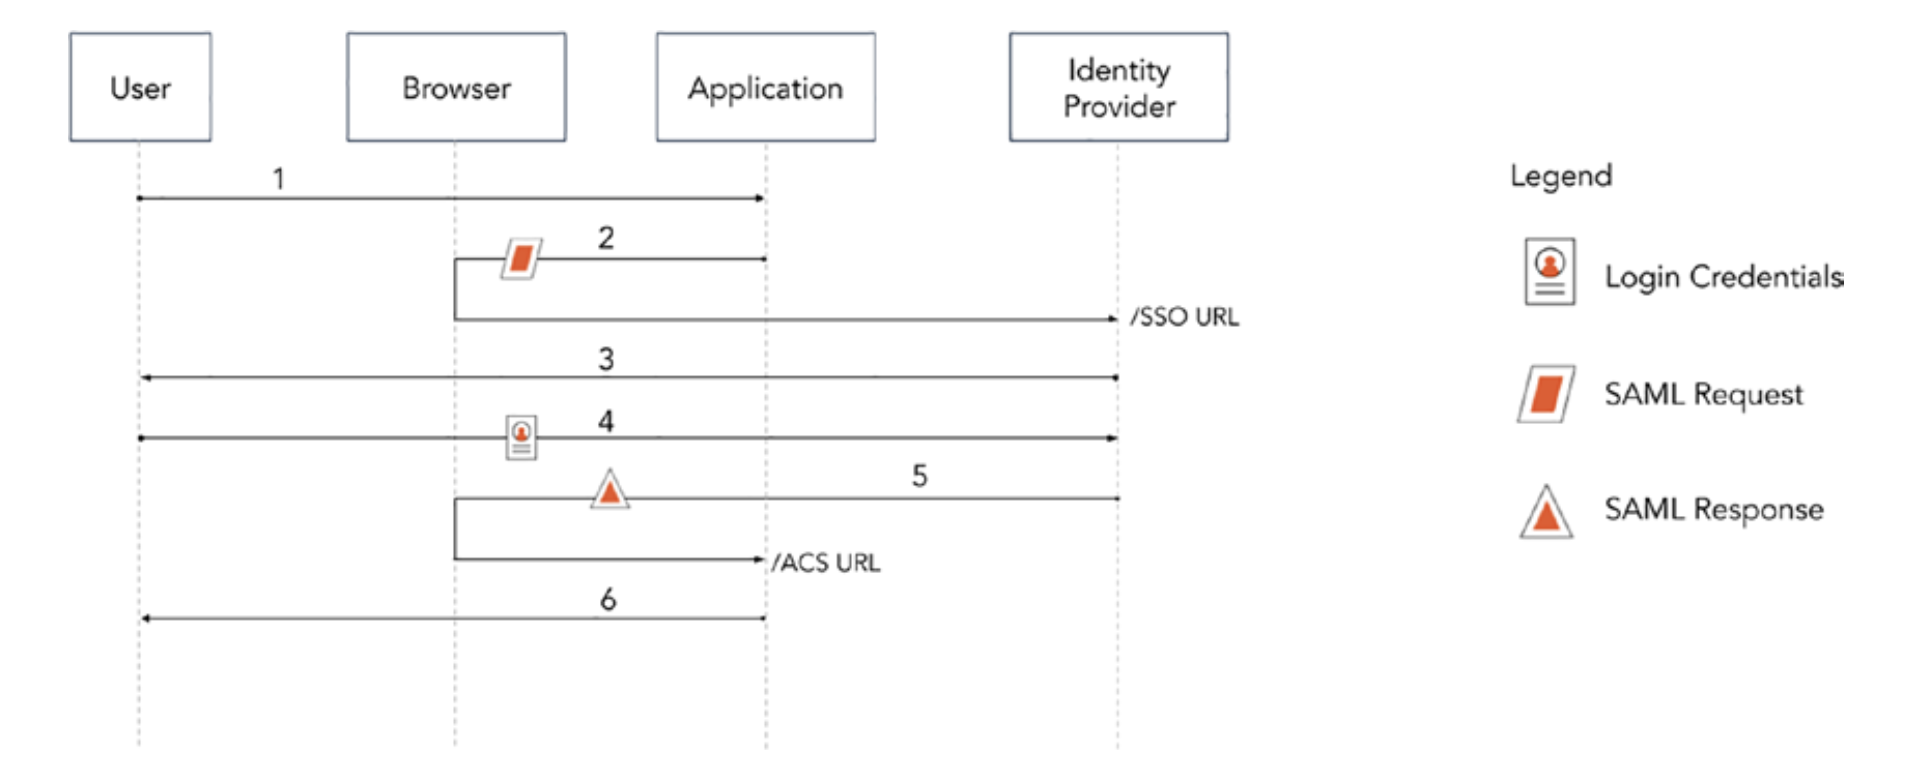
\includegraphics[width=0.8\textwidth]{../img/SP-initiated-flow.png}
  \caption{SP initiated flow} 
  \label{saml_sp_initiated}
\end{figure}

Additionally, the IdP can be a corporate application of the university. If the student is connected to that corporate application and want to access his online student account, the student will not be asked to reauthenticate and will be automatically granted access to the requested resource. This is called IdP initiated flow (Figure \ref{saml_idp_initiated}), as the authentication process is initiated by the identity provider, rather than the service provider. In this flow, the user first authenticates with the IdP, and then the IdP initiates the SAML assertion to the SP to grant access to the requested resource.

\begin{figure}[htp]
  \centering
  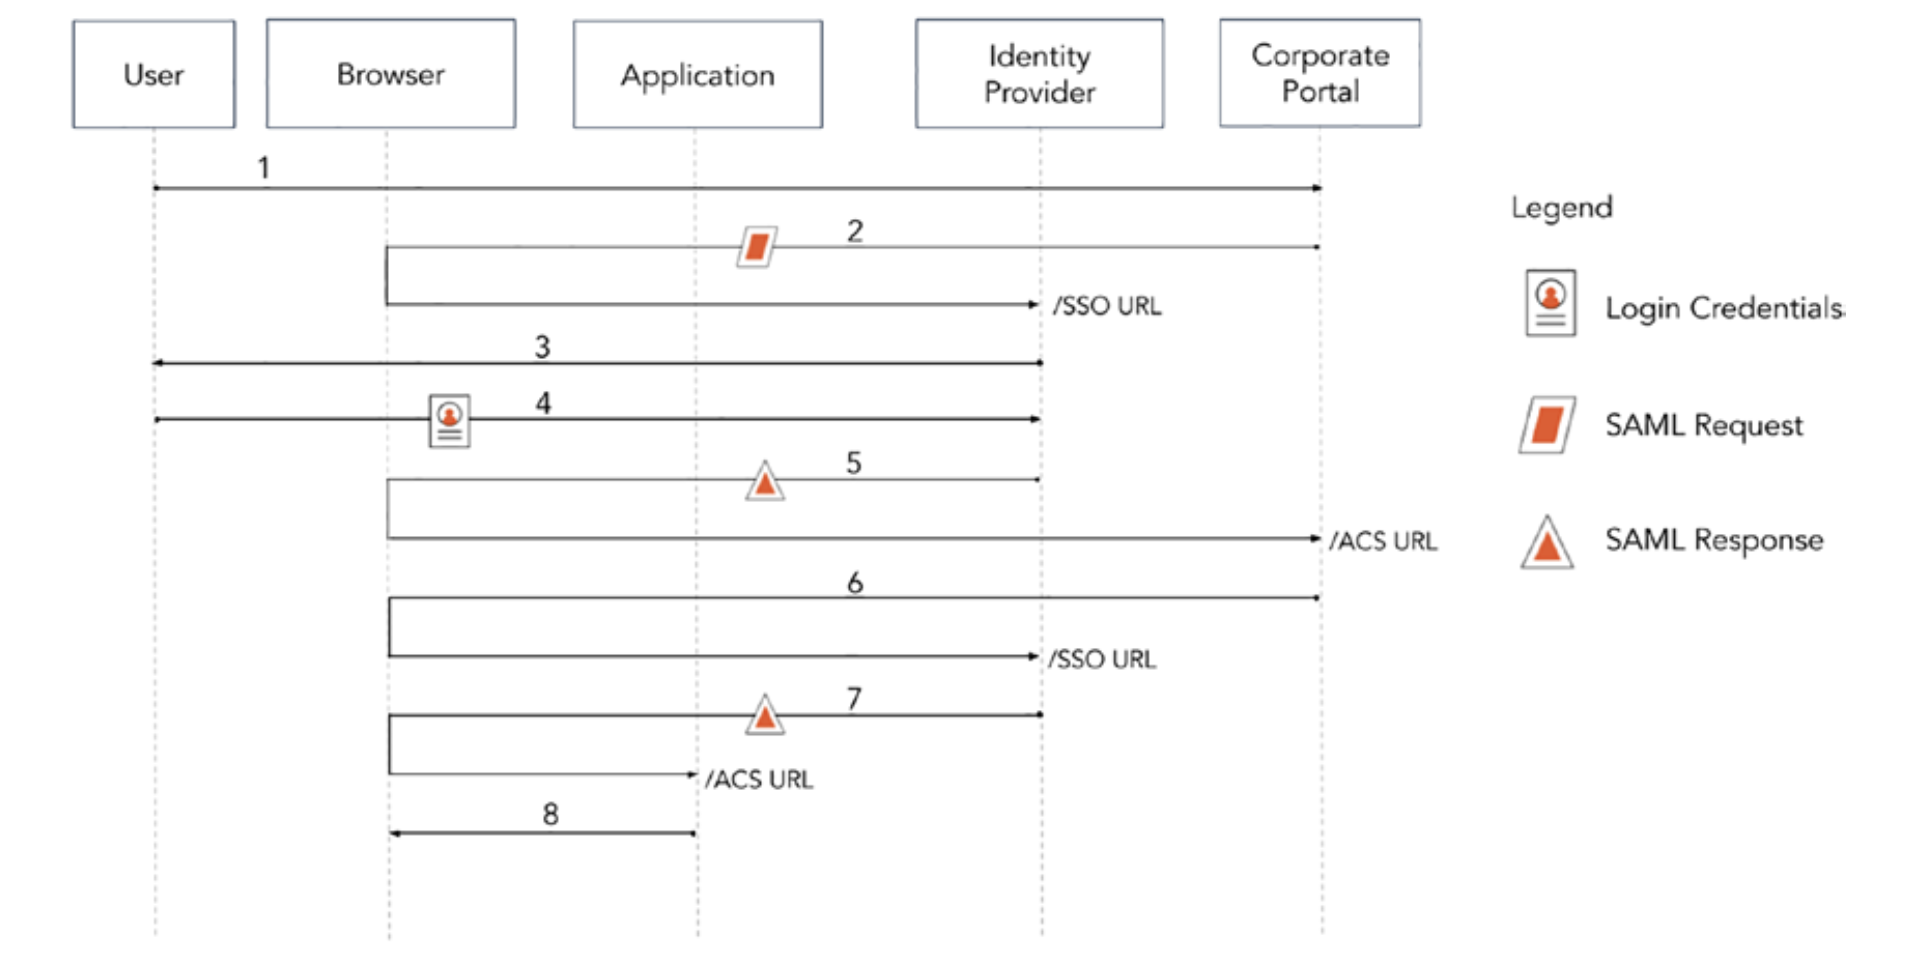
\includegraphics[width=0.8\textwidth]{../img/IdP-initiated flow.png}
  \caption{IdP initiated flow \cite{wilson2022}}
  \label{saml_idp_initiated}
\end{figure}

SAML is built such that every message between the SP and IdP transits via the user agent (browser). These SAML requests and responses are transmitted through binding mechanisms such as HTTP POST, typically used when the assertion is signed and voluminous, or HTTP Redirect, generally employed when the assertion are shorter and not signed \cite[p.~347]{wilson2022}. 


\subsection{OAuth 2.0}

While SAML implements two flows, OAuth 2.0 has additional flows depending on the type of client application and the level of security required.

Moreover, unlike OAuth 1.0, OAuth 2.0 does not specify a single flow to treat all use cases, but rather defines several flows, each designed for specific scenarios \cite[p.~93]{richer2017}.

\subsubsection*{Authorization Code Flow}

This is the commonest flow used for web applications and mobile applications. In this flow, the client application(CA) want to act on behalf of the user to access protected resources stored at the resource server (RS). So, the CA redirects the user to the AS to authenticate and authorize the CA to access the user's resources. After successful authentication and authorization, the authorization server returns an authorization code to the CA, which then exchanges it for an access token by authenticating itself to the AS and presenting the authorization code. This flow provides a high level of security as the access token is never exposed to the user agent and is only transmitted between CA and AS through secure back-channel communication and CA never see the user credentials. Additionally, refresh tokens are issued in this flow to allow long-term access without requiring the user to reauthenticate. Each step of this flow is designed in Figure \ref{oauth_code_grant}.

\begin{figure}[htp]
  \centering
  \includesvg[width=0.9\textwidth, inkscapelatex=false]{../img/oauth_code_grant}
  \caption{OAuth 2.0 Authorization Code Grant Flow \cite[p.~23]{richer2017}}
  \label{oauth_code_grant}
\end{figure}

\subsubsection*{Authorization Code Flow with Proof Key Code Exchange (PKCE)}

This flow is an extension of the Authorization Code Flow and it was designed to add an additional layer of security and to allow SPA to use OAuth as they can not store securely the client secret. In this flow, the CA generates a random string called a "code verifier" and derives a "code challenge" from it by using a transformation method (e.g., SHA-256). When the CA initiates the authorization request via the front channel, it includes the code challenge in it. After the user authenticates and authorizes the CA, the AS returns an authorization code to the CA. The CA then authenticates itself and exchanges the authorization code and the original code verifier for an access token. The AS compares the code verifier with the code challenge by applying the same transformation method to the code verifier and checking if it matches the code challenge. If they match, the AS issues an access token. A refresh token is also issued in this flow to allow long-term access without requiring the user to reauthenticate. The Figure \ref{pkce_flow} illustrates this flow step by step.

\begin{figure}[htp]
  \centering
  \includesvg[width=0.9\textwidth, inkscapelatex=false]{../img/pkce_flow}
  \caption{Authorization Code Grant with PKCE Flow \cite[p.~177]{richer2017}}
  \label{pkce_flow}
\end{figure}

\subsubsection*{Implicit Flow}

This flow is designed for client applications that run entirely within a browser, such as Single-Page Applications (SPAs). Since any secret stored directly in JavaScript code would be accessible to everyone, the access ttoken is returned directly to the client without an intermediate authorization code exchange. This approach removes the security protections associated with non-repudiation. Furthermore, refresh tokens are not issued in this flow, as these applications are generally used for short-lived access and lack the infrastructure to securely store long-term credentials. This is dangerous and it has been removed in the latest version of OAuth 2.1 \cite[p.~116]{wilson2022}\cite{rfc9700}.

\subsubsection*{Client Credentials Flow}

This flow is intended for server-to-server communication, where the client application is a confidential client (dark, and secure backend server) that can securely store its credentials. In this flow, the client application directly authenticates with the authorization server using its own credentials (client ID and client secret) to obtain an access token. Since the client can request the token whenever he wants by just providing his credentials, the refresh token is no longer needed. This flow does not involve user authentication, as it is designed for scenarios where the client application needs the access in the resource server on behalf of itself rather than on behalf of a user.


\subsubsection*{Resource Owner Credentials Flow}

This flow is used when it exists no other viable solution than this. In this flow, the user provides their credentials (username and password) directly to the client application, which then uses these credentials to obtain an access token from the authorization server in the back channel. So, the refresh token is not needed in this flow as the client can request the token whenever he wants by just providing the user credentials in HTTP POST request. Furthermore, the resource server does not have to see the user credentials. However, it is generally discouraged due to security concerns, as it requires users to share their credentials with the client application, which can lead to potential security risks if the client application is compromised.

\subsubsection*{Assertion Grant Types}

In this flow, the client application can obtain an access token by presenting an assertion to the authorization server. The assertion can be handed in different formats, such as SAML assertions or JSON Web Tokens (JWTs). The client application can obtain the assertion from an external identity provider or generate it itself or through another non-OAuth protocol. Furthermore, the client uses his credentials (client ID and client secret) and the assertion to authenticate with the authorization server and request an access token. And, based on the assertion, the right scope of access is determined by the authorization server. Since it rely on the back channel communication between the client and the authorization server, and a user is not involved in this flow, the refresh token is not required.


\subsubsection*{Device Authorization Flow}

This flow is designed for devices that do not have a browser or have limited input capabilities, such as smart TVs, gaming consoles, or IoT devices\cite{rfc8628}. In this flow, the device initiates the authorization process by requesting a device code and a user code from the authorization server. The device then displays the user code to the user and instructs them to visit a specific URL on another device (e.g., a smartphone or computer) to enter the user code and authenticate. Once the user successfully authenticates and authorizes the device, the authorization server issues an access token to the device in response to the polling requests repeatedly send by the device on the waiting period. Since the device can request the token whenever he wants by just providing the user code, the refresh token is not needed in this flow.

\subsection{OIDC}

Since OIDC is built on top of OAuth 2.0, it consequently inherits all its flows. However, OIDC is designed to provide an authentication layer, so it independently override some flows to integrate the authentication requirements. These flows are: the Authorization Code Flow, the Implicit Flow, and the Hybrid Flow \cite[p.~109]{wilson2022}\cite[p.~5]{yildiz2026}, the Client-Initiated Backchannel Authentication Flow (CIBA) \cite{wilson2022}\cite{ciba}.

\subsubsection*{Authorization Code Flow}

This flow works similarly to the OAuth 2.0 Authorization Code Flow, but with the addition of an ID token that is returned by the OP (AS) along with the access token. Consequently, it also works for the authorization code flow with PKCE. 

\subsubsection*{Implicit Flow}

This flow is also similar to the OAuth 2.0 Implicit Flow. But in this case, the ID Token is returned directly to the CA after the user authenticates on the OP. However, since an application that only needs to authenticate users does not need to obtain an access token, this flow can be tolerated if the access token is not issued\cite[p.~116]{wilson2022}. Even though, \cite{rfc9700}\cite{oidc_core} strictly discouraged to use this flow as it exposes the access token to the user agent. 

\subsubsection*{Hybrid Flow}

This flow is a combination of the authorization code flow and the implicit flow. Specifically, the CA can request the authorization code and optionally one or more additional parameters (ID token, access token, or both) in the initial authorization request\cite{oidc_core}\cite[p119]{wilson2022}. This allows the CA to obtain an ID Token and the authorization code in the front channel, while still using the authorization code flow to obtain an access token securely in the back channel. However, the CA can but should not request the access token in the front channel as it is not a good practice\cite{oidc_core}\cite{rfc9700}.

\subsubsection*{Client-Initiated Backchannel Authentication Flow (CIBA)}


This flow is designed for scenarios where the client application cannot directly interact with the user, such as in the case of a command-line interface or a voice assistant. It enables the client application to initiate the authentication of the end-user through a different channel.


In this flow, the client application initiates the authentication process by sending an authentication request to the OP through a back channel communication. The OP then prompts the user to authenticate using a separate device, such as a smartphone or computer. Once the user successfully authenticates, the OP sends an authentication response to the client application through the back channel, which includes an ID token and optionally an access token. This flow allows for secure authentication without requiring direct user interaction with the client application.

\subsection{Flows decision graph}

\begin{comment}
\subsubsection*{Flow decision graph}

Considering these flows, when implementing OAuth 2.0, the choice of the flow should be based on the Figure \ref{oauth_flow_choice}. 

\begin{figure}[htp]
  \centering
  \includesvg[width=\textwidth, inkscapelatex=false]{../img/oauth_flow_choice}
  \caption{Choosing the right grant type \cite[p.~108]{richer2017}}
  \label{oauth_flow_choice}
\end{figure}
\end{comment}


\section{Token formats and structures}

SAML, OAuth 2.0 and OIDC use different token formats and structures to represent the authentication and authorization information. In the following sections, we will describe the different token formats and structures of each protocol and compare them in a synthetic table at the end of this section.


\begin{comment}
  2.1. Architecture et flux d'authentification/autorisation
    - Flows SAML : SP-initiated vs IdP-initiated
    - Flows OAuth 2.0 : Authorization Code, Client Credentials, etc.
    - Flows OIDC : héritage OAuth + ID Token
    > Tableau comparatif synthétique

  2.2. Formats et structures des tokens
      - SAML : assertions XML signées
      - OAuth 2.0 : tokens opaques ou JWT
      - OIDC : ID Token JWT standardisé
      > Analyse taille, parsing, validation
      
  2.3. Mécanismes de sécurité
      - SAML : signatures XML, PKI, encryption
      - OAuth 2.0 : PKCE, state, HTTPS
      - OIDC : nonce, at_hash, algorithmes signature
      > Comparaison vulnérabilités et mitigations (appui sur arXiv)
      
  2.4. Gestion des sessions et révocation
      - SAML : SSO, Single Logout
      - OAuth 2.0 : refresh tokens, révocation RFC 7009
      - OIDC : session management, logout flows
      > Matrice de comparaison

  OAUTH 2.0

  Firstly, when a ressource owner (RO) want to grant access to a client application, the client redirects him to an authorization endpoint via an HTTP Redirect request. 

  Additionnally, authorization server(AS) in response triggers an authentification process to the user (this part is independent of the protocol, as the authentification method is not standardized by OAuth2.0), following the success authentification of the user, an autorization code is grant to the client application by the AS in an HTTP Redirect response.

  Moreover, the client application authenticates itself to the AS and present the autorization code to act on behalf the RO via an HTTP POST with the parameters encoded as a form HTTP. This authentification are made seperately and only between each actor to prevent the the other actor to see the credentials of the other.

  Finally, the AS sends an access token to client, and the client uses that token to access ressources stored at the ressource server(RS). The client use the token as an opaque key because it does not have to see what is inside the token. He only have to present it to the ressource server.


  \begin{figure}[htp]
    \centering
    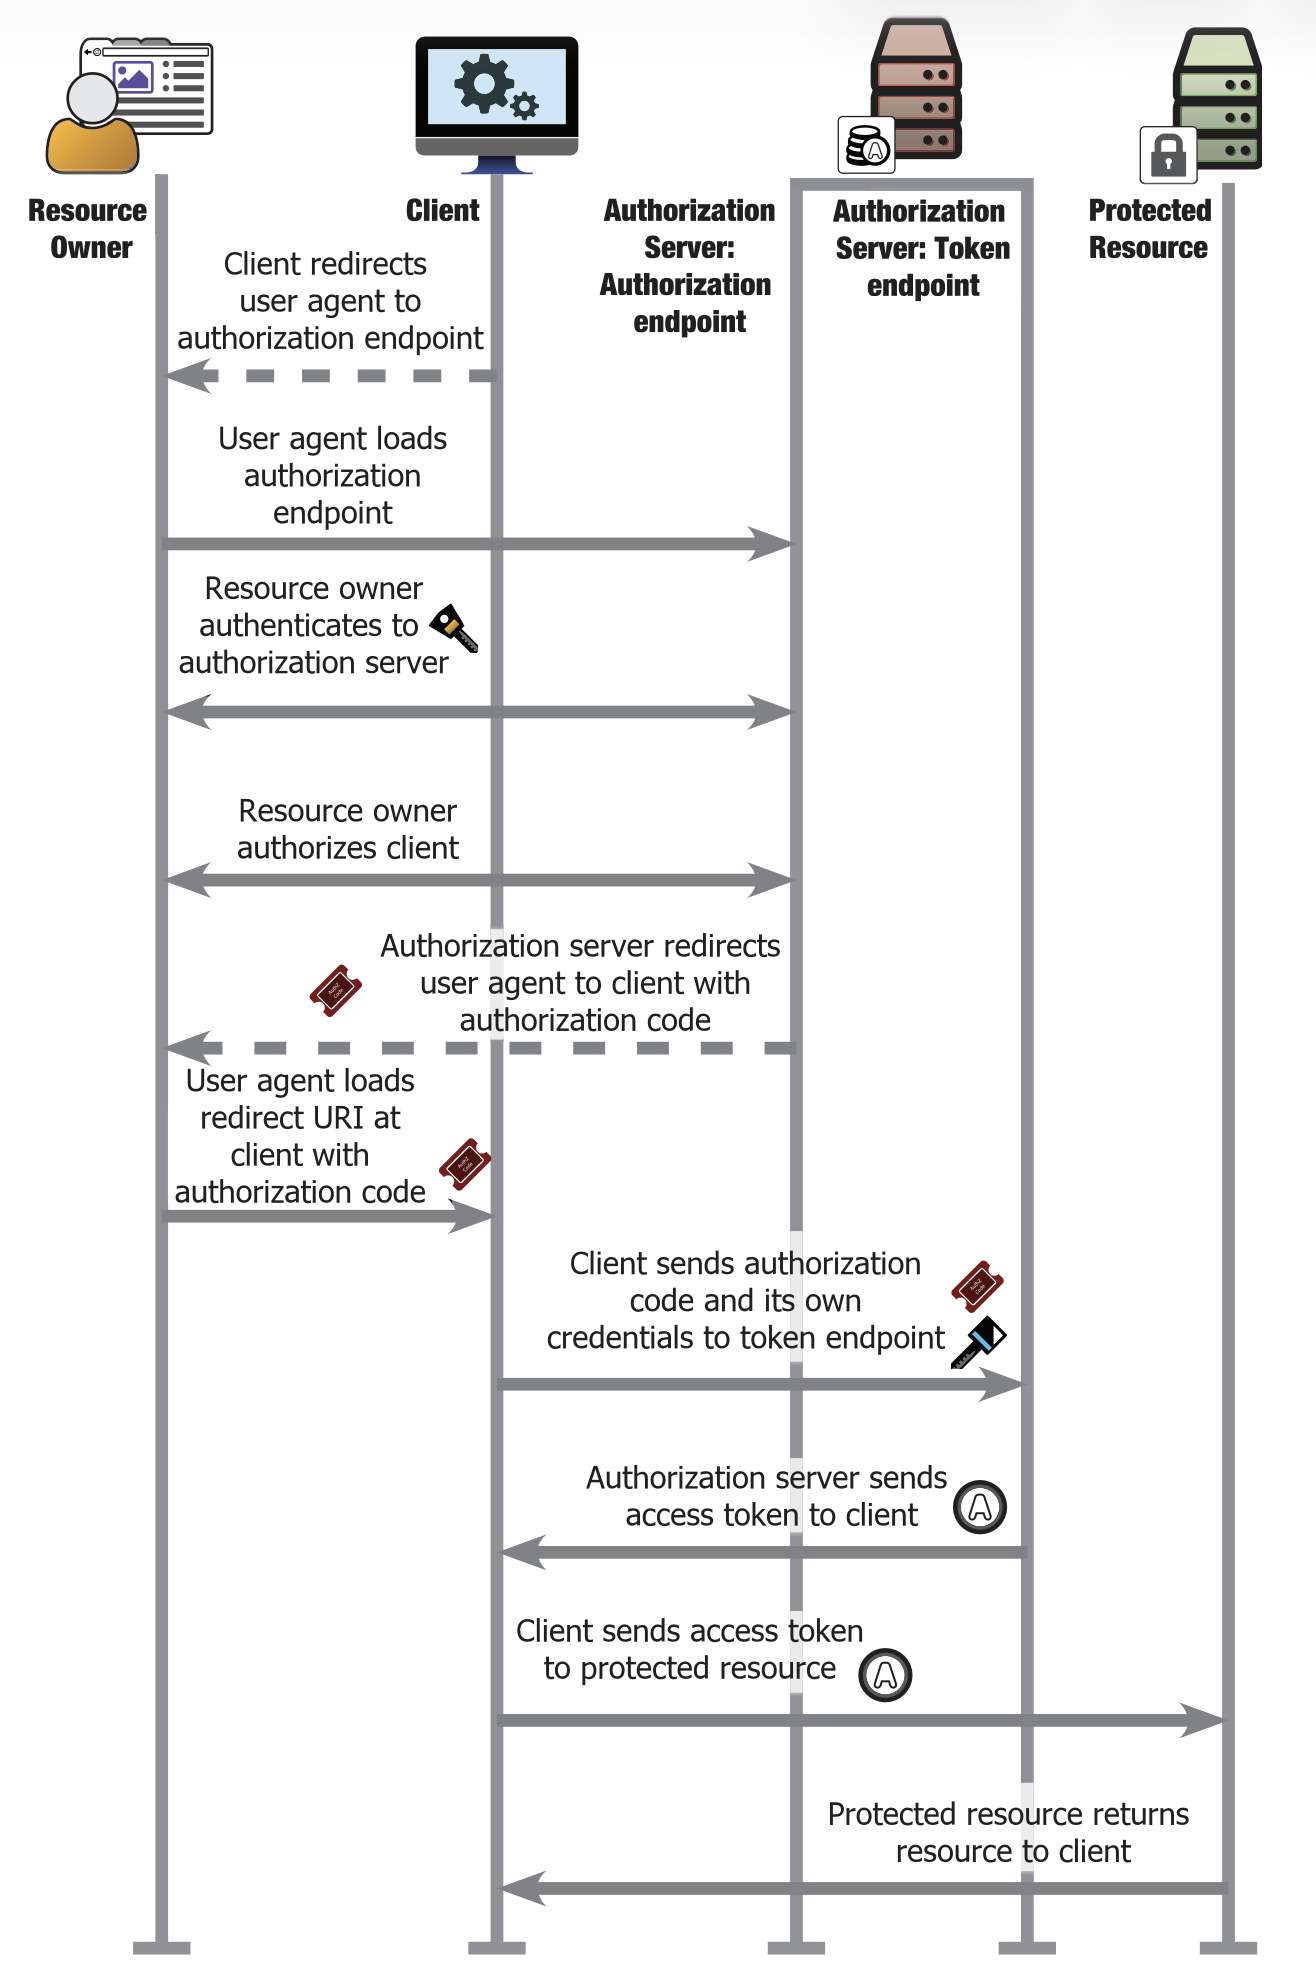
\includegraphics[width=0.8\textwidth]{../img/oauth_code_grant.png}
    \caption{OAuth 2.0 Authorization Code Grant Flow \cite{richer2017}}
    \label{oauth_code_grant}
  \end{figure}


  OIDC

  For example, when signing up to an application nowadays, it exists many possibilities like providing username, password, or sign in with your Google account. Particularly the "Sign up with Google Account" button is the trigger of the OIDC mechanism.

  When clicking on the latter button, the browser redirect the user to the Google authentication page, where the user will be asked to provide his credentials. After successful authentication, Google will send an ID token to the client application, which is used to create the user account. The client application can also obtain an access token to access protected resources on behalf of the user like OAuth 2.0. This allows the client to store minimal user information in a session or access protected ressources on behalf of the user. The OIDC provider (Google in this case) is in charge of the securization of the sensitive data of the users. 

  Basically, the Figure \ref{oidc_overview} pictures the require actors to make OIDC work.

  \begin{figure}[htp]
    \centering
    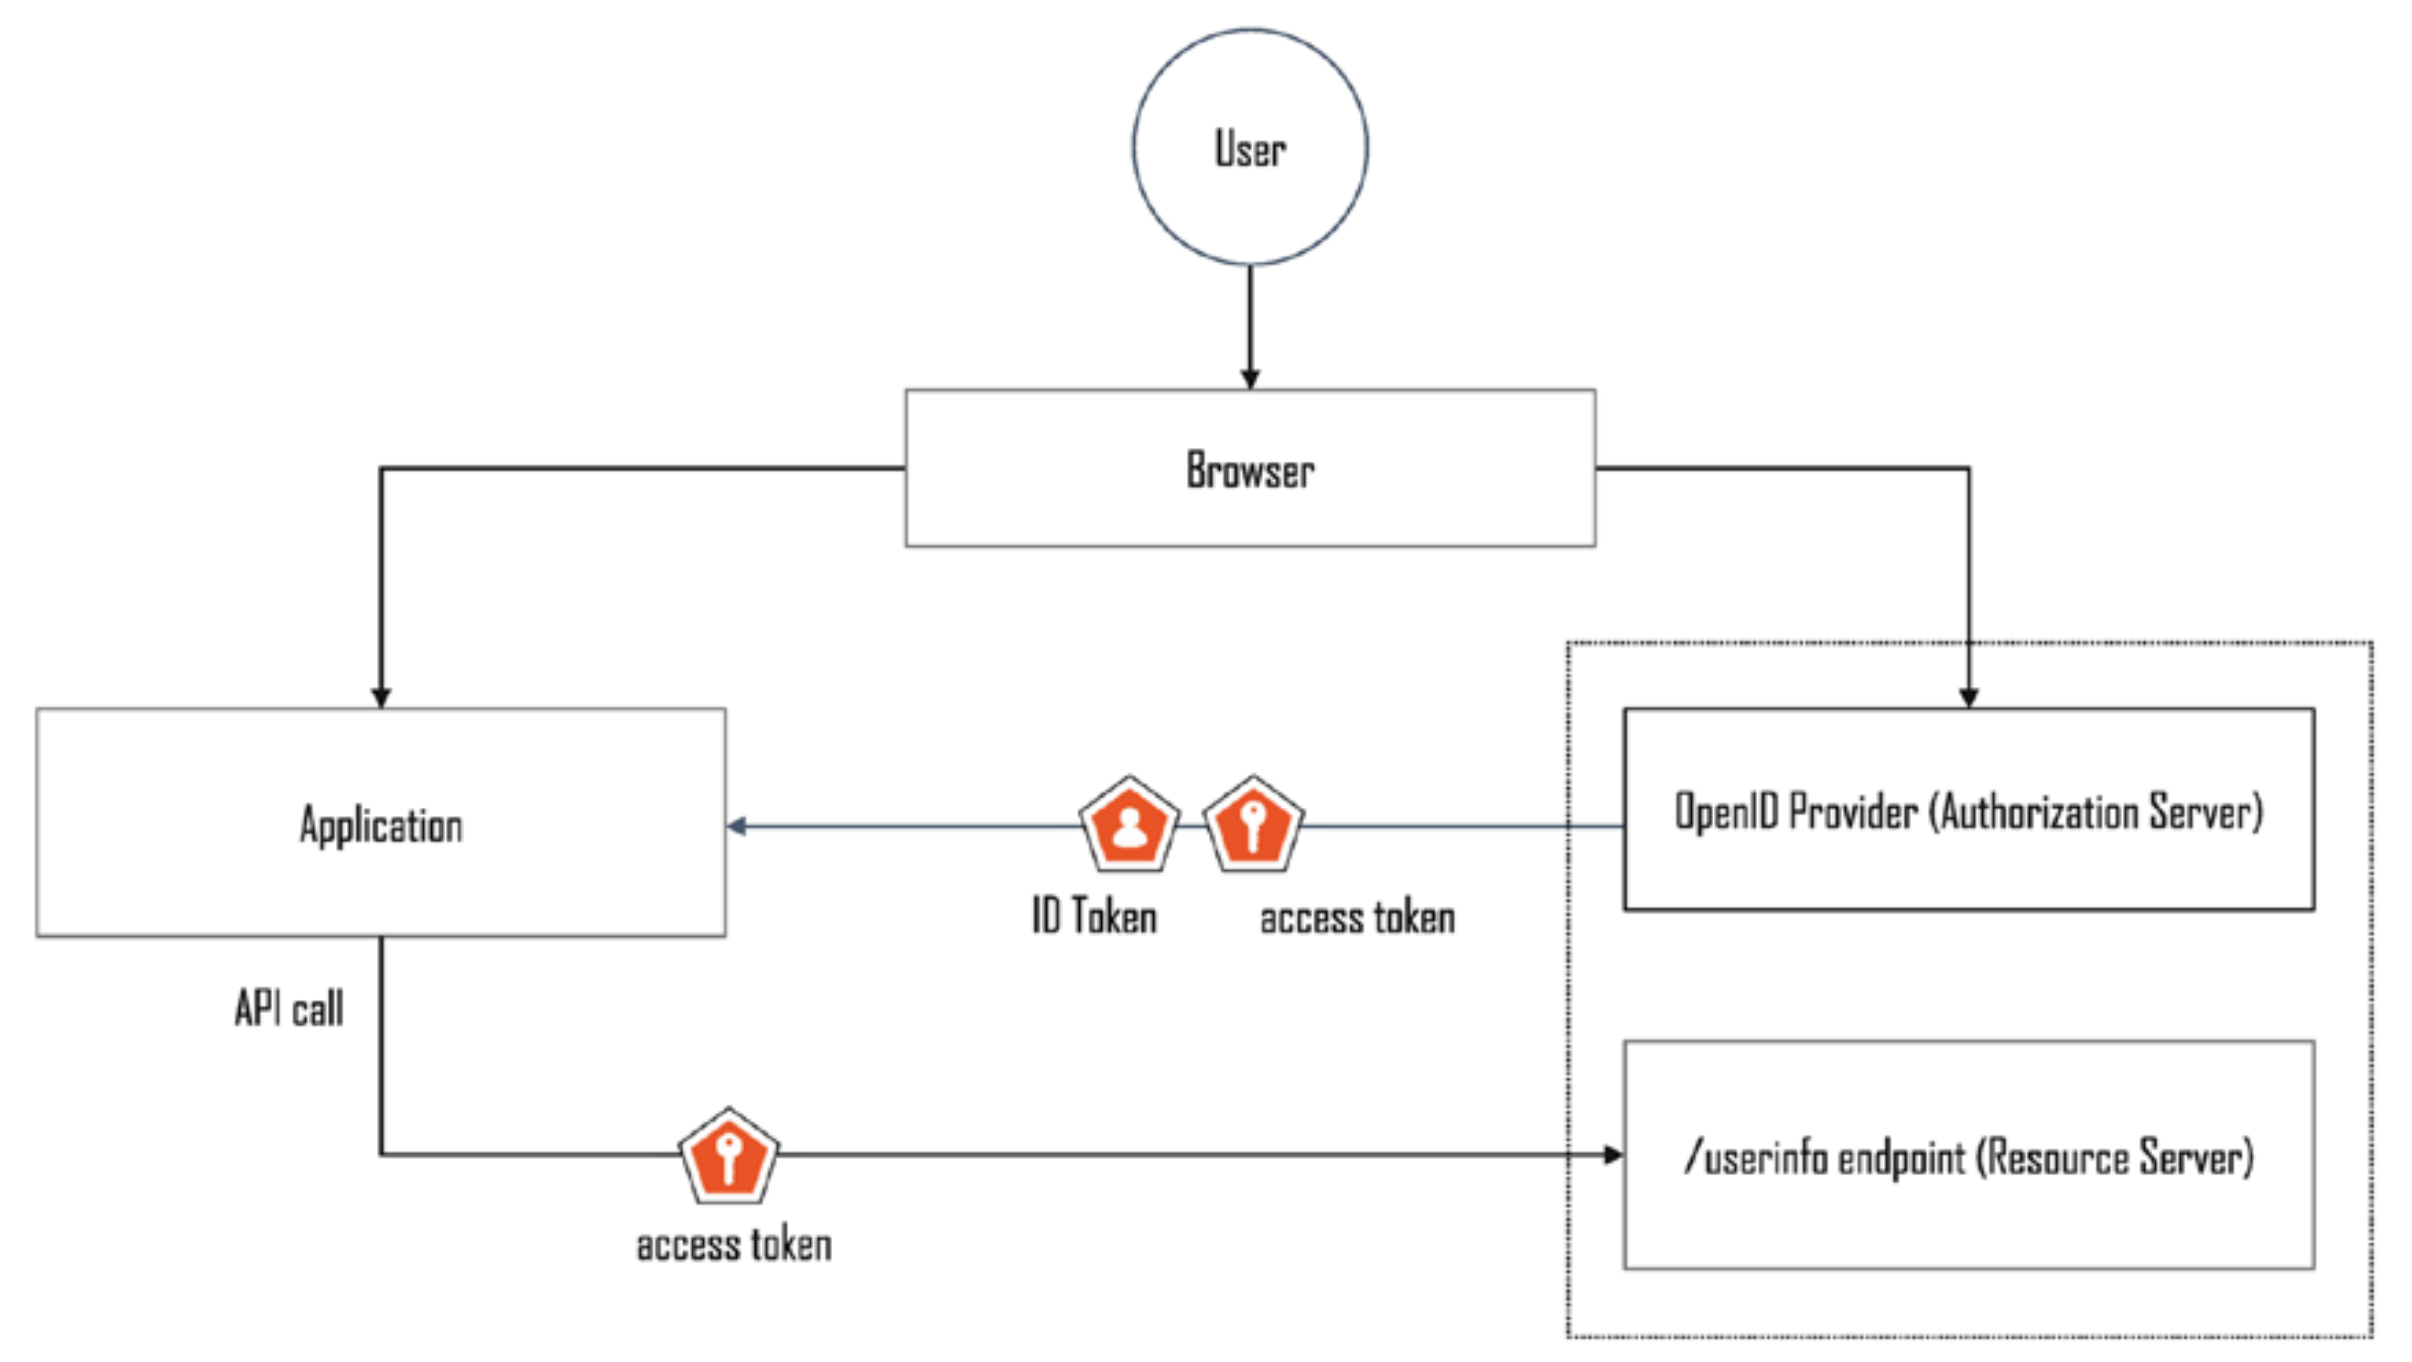
\includegraphics[width=0.8\textwidth]{../img/oidc-overview.png}
    \caption{OIDC overview \cite{wilson2022}}
    \label{oidc_overview}
  \end{figure}



  SAML

\end{comment}


\end{document}

